\section{Adaptiv}

Gennem Design sektionen, kommer vi ikke ind på den adaptive del af projektet. Dette skyldes grundet tidsmangel, at gruppen ikke nåede at implementere et adaptiv regulerings feedback. I dette afsnit, vil der forklares om adaptiv controller, og hvordan det burde være implementeret til projektet. 

Problemene med et normalt kontrolsystem er, at dele af systemet kan være ukendt eller have ukendte parametre. Systemets parametre kan ofte varierer med tiden (slid på dæk, mindre vægt osv.), og systemet kan blive påvirket af ukendte forstyrrelser (støj, vind, varme), som ændre systemet karakteristik. Derfor indfører man ofte en adaptiv controller til at tilpasse sig ændringerne og til at ændre systemets adfærd til at overholde nye omstændigheder.
Følgende to regulatorer er eksempler på adaptive regulatorer, som kan løse overstående problemer.  


\subsection{MRAC regulator}
Model Reference Adaptive Control (MRAC) er en adaptiv regulator model, som bygger på en reference model af systemet.
MRAC designes normalt til at oprette en closed-loop controller med opdaterende parametre til at ændre systemets respons som ønsket. I modellen sammenlignes udgangen af systemet med et ønsket svar fra en referencemodel, og opdateringen af kontrol parametrene er baseret på denne fejl. Formålet med disse parametre er at matche de ønskede værdier, således at systemet output matcher referencemodellens output \cite{adaptive}.
Herunder vises hvordan et klassisk MRAC system ser ud:


\begin{figure}[H]
	\centering
	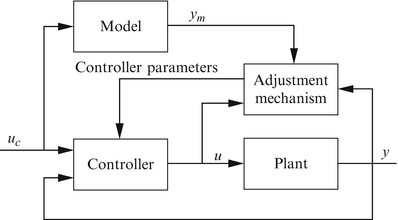
\includegraphics[width = 300pt]{figur/MRAC}
	\caption{Klassisk MRAC system}
	\label{fig:MRAC}
\end{figure}

For at bestemme den adjustment mechanism, som skal bringe fejlen mellem systemets output og referencemodellens output bruger man ofte den såkaldte MIT rule. MIT rule er en måde at beregne de adjustment mechanism, som vist på \autoref{fig:MRAC}, som skal til for at systemet opfører sig adaptiv. MIT-reglen kan betragtes som en gradient løsning for at minimere den kvadratiske fejl $e^{2}$. For at sikre stabilitet, kan den modificerede MIT rule benyttes. Dette gøres, hvis reference inputtet har store udsving, som kan gøre systemet ustabil. \\


\subsection{MIAC}
Til dette projekt, skulle der have været en adaptiv regulering, og derigennem var valget faldet på at bruge Model Identification Adaptive Control (MIAC). Ideen med et MIAC system er regulatoren hele tiden står og identificere processen, som kører ved hjælp af en estimator. Herefter gendesigner regulatoren selve controllerens parametere ud fra den fundne system model og kravene til responsen for systemet. Dette gør, at hvis systemets parametre har ændret sig i forhold til startparametrene, så tuner regulatoren selv centrolleren ind til de nye system parametre. Derfor kaldes denne type controller også ofte Self-tuning-regulator \cite{adaptive}. En anden fordel ved systemet er, at hvis det oprindelige controller design ikke passer helt med den reelle process, så tuner regulatoren også langsomt det delvist forkerte controller design ind til den ønskede respons. Herunder vises hvordan et klassisk MIAC system ser ud:

\begin{figure}[H]
	\centering
	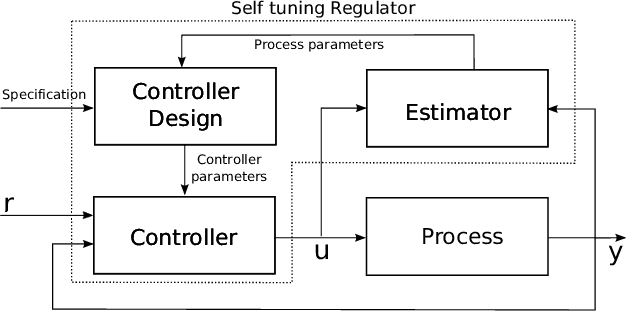
\includegraphics[width = 300pt]{figur/MIAC}
	\caption{Klassisk MIAC system}
	\label{fig:MIAC}
\end{figure}

\subsubsection{RLS}
Til MIAC skal der benyttes en estimation mekanisme, og derigennem blev der valgt at bruge Recursive least squares (RLS) algoritmen, da vi havde kendskab til denne metode gennem undervisningen, og fordi den er nem at tilgå. Her skulle systemets estimation mekanisme laves ud fra online RLS, da systemet skal kunne køre i reel tid og derfor ikke har et hele udgangssignalet for processen. 

RLS algoritmen er en adaptiv filteralgoritme, der recursivt finder koefficienterne(estimation), der minimerer en vægtet lineær least squared kostprisfunktion i forbindelse med indgangssignalerne versus udgangssignalerne. Til realiseringen af det adaptive system, var planen at indsætte RLS algoritmen i system estimator blokken, som ses på \autoref{fig:MIAC}. Hertil skulle der laves en regulerings blok, som regulerede på K værdierne i forhold til de valgte specifikationer som på \autoref{fig:Blokdiagram}.
RLS algoritmen, ville levere en estimation af systemet Thetahat. RLS algoritmen kan ses i \autoref{fig:RLS_formel} 


 \begin{figure}[H]
	\centering
	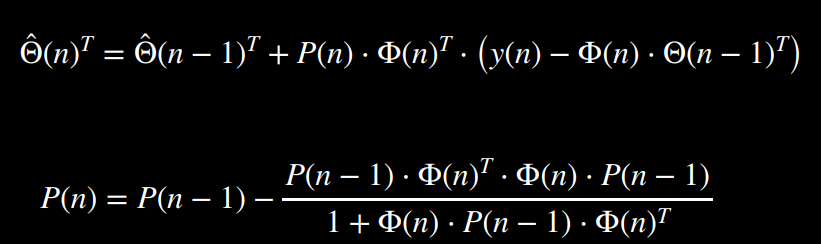
\includegraphics[width = 300pt]{figur/RLS_formel}
	\caption{Formel for theta fra RLS online blokken}
	\label{fig:RLS_formel}
\end{figure}
Hvor Phi de kendte værdier, in- og output sat sammen i en samlet vektor,  mens Thetahat er model parmenterne for systemet (estimation) sat sammen i en samlet vektor 

\subsubsection{Glemselsfaktor og Kalman filter}  
Det endelige RLS system kan forbedres med flere faktorer, her vil vi kort forklare om de to tilføjelser, som er blevet præsenteret til undervisningen, og som RLS algotirmen kan udvides med.

\textbf{Glemselsfaktor}
Glemselsfaktoren gør det, at modellen kigger mere på de forrige samples end de tidlige, og derfor ikke kigger jævnt  på hele signalet. Dette gør systemet hurtigere overfor ændringer, da den nye sampling med ændringen vejere tungere end tidligere samples. Dette fjerne modelstøjen fra estimationen, hvis processens karatestik er tidsafhængig. 

\textbf{Kalman filter}
RLS antager, at der ikke er noget målestøj, og at det vi måler præcis er input og output. Kalman filteret er godt i de situationer, hvor der tilføres støj til systemet, som reelt set altid vil være i en virkelig implementering. Her er Kalman filteret ikke så modtagelig overfor støj, og derved bedre til at estimere de korrekte værdier end standard RLS.

